\documentclass{article}%
\usepackage[T1]{fontenc}%
\usepackage[utf8]{inputenc}%
\usepackage{lmodern}%
\usepackage{textcomp}%
\usepackage{lastpage}%
\usepackage{authblk}%
\usepackage{graphicx}%
%
\title{Regulation of MYC Expression and Differential JQ1 Sensitivity in Cancer Cells}%
\author{Kathryn Brown}%
\affil{Department of Comparative Physiology, Uppsala University, Uppsala, Sweden}%
\date{01{-}01{-}2014}%
%
\begin{document}%
\normalsize%
\maketitle%
\section{Abstract}%
\label{sec:Abstract}%
The dangers of exposing humans to collagen three{-}hydroxylation {-}{-} this is the process where 3{-}H of the firm bonding enzyme fatty acids are extracted and then used as a cleaner {-}{-} can lead to a mixture of metals in a porous bone.\newline%
Use of this process {-}{-} also known as 3{-}H2O reductase 3{-}h2O {-}{-} is only routine for the removal of bone plaque. The problem occurs when people use the paste to use at a medical facility for toxic bacteria like Staphylococcus Aureus, for example.\newline%
Were not saying you should stop using collagen three{-}hydroxylation to remove bacteria, no. And, there are certain procedures that require contact with this enzyme. However, Dr. Anupam Pawar, the chief of orthopedic surgery at UCSF Benioff Childrens Hospital San Francisco, strongly suggests against using 3{-}H2O reductase 3{-}h2O for certain abnormal injuries or pain conditions.\newline%
Pawar tells us, I think the important thing to take away from this is that my patients are taking very serious care of their bone. The strongest evidence to date is that the very mild symptomatic pain thats caused by H2O reductase 3{-}h2O cannot be treatable.\newline%
According to a 2008 Johns Hopkins Medicine study, patients with pain associated with shock that wasnt due to an injury, bone damage, illness or cancer had the highest chances of recovering with high pressure H2O reductase 3{-}h2O. However, while exposure is an issue, Parkinsons Disease does not appear to be linked to H2O reductase 3{-}h2O usage.\newline%
Besides these risks, H2O reductase 3{-}h2O actually enhances pain relief in patients who have pain related to a fracture or stroke. The idea, Pawar says, is that H2O reductase 3{-}h2O will leave patients with less tension on the bones so they can get the pain relief thats usually associated with a period of bruising or bursitis.\newline%
Still, Pawar says that H2

%
\subsection{Image Analysis}%
\label{subsec:ImageAnalysis}%


\begin{figure}[h!]%
\centering%
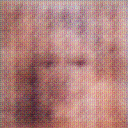
\includegraphics[width=150px]{500_fake_images/samples_5_131.png}%
\caption{A Black And White Photo Of A Black And White Photo}%
\end{figure}

%
\end{document}